\documentclass[border=8pt]{standalone}
\usepackage{ctex}
\usepackage{amssymb}
\usepackage{tikz}
\usetikzlibrary{arrows.meta}

\begin{document}
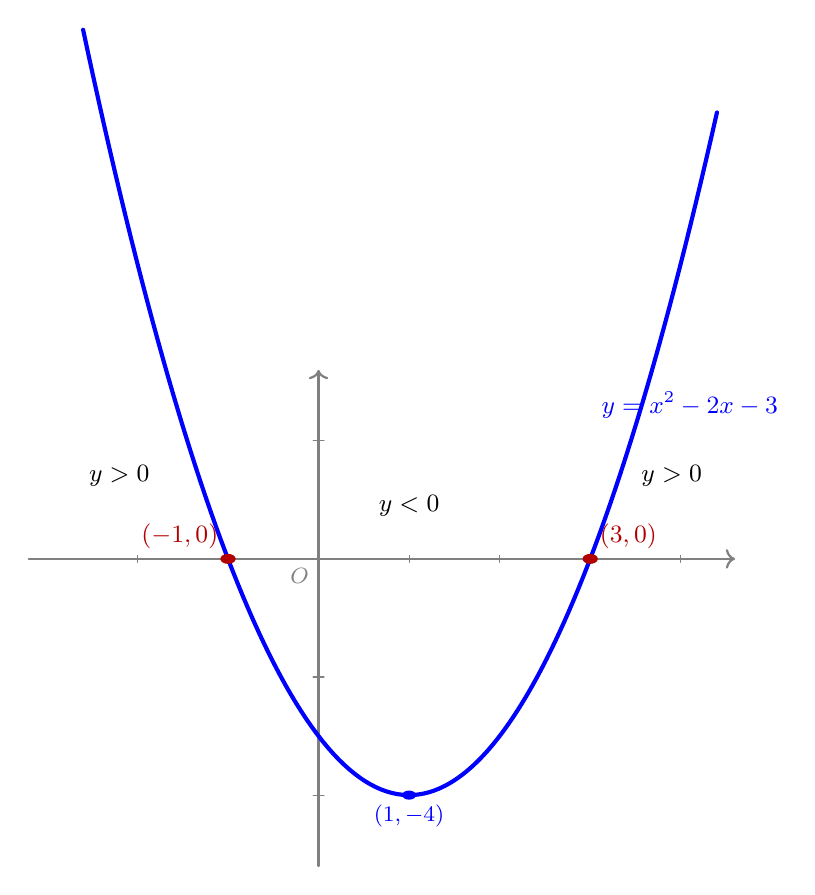
\begin{tikzpicture}[xscale=1.15, yscale=0.75, line cap=round, line join=round]

% 坐标轴
\draw[->, gray, line width=0.8pt] (-3.2,0) -- (4.6,0);
\draw[->, gray, line width=0.8pt] (0,-5.2) -- (0,3.2);
\node[gray, below left, font=\footnotesize] at (0,0) {$O$};

% 数轴刻度
\foreach \x in {-2,-1,1,2,3,4} \draw[gray] (\x,0.06) -- (\x,-0.06);
\foreach \y in {-4,-2,2} \draw[gray] (0.06,\y) -- (-0.06,\y);

% 抛物线 y = (x-3)(x+1)
\draw[blue, line width=1.5pt, domain=-2.6:4.4, samples=120]
  plot(\x, {(\x-3)*(\x+1)});

% 顶点
\fill[blue] (1,-4) circle (2.2pt);
\node[blue, below, font=\footnotesize] at (1,-4) {$(1,-4)$};

% 与 x 轴交点
\foreach \x in {-1,3} {
  \fill[red!70!black] (\x,0) circle (2.4pt);
}

% 方程：交点
\node[red!70!black, above left, font=\small] at (-1,0) {$(-1,0)$};
\node[red!70!black, above right, font=\small] at (3,0) {$(3,0)$};

% 标注
\node[blue, font=\small] at (4.1,2.6) {$y=x^2-2x-3$};

% 上方区域（>0）
\node[font=\small] at (-2.2,1.4) {$y>0$};
\node[font=\small] at (3.9,1.4) {$y>0$};

% 下方区域（<0）
\node[font=\small] at (1,0.9) {$y<0$};

\end{tikzpicture}
\end{document}
